\begin{figure}

\setlength{\unitlength}{\textwidth}
\fbox{
  \begin{picture}(1,0.3)(0.0,0.45)
    
       \put(0.025,0.5){\includegraphics[width=0.5\unitlength]{../FnP/gnuplot/mean_power_collapsed_mstar.eps}}
       \put(0.495,0.5){\includegraphics[width=0.5\unitlength]{../FnP/gnuplot/mean_power_collapsed_noshed_mstar.eps}}
       
        
        \put(-0.01,0.637){\large $\frac{P_{m}}{\rho \mathcal{A}U^3}$}
              
        \put(0.23,0.48){$\displaystyle\frac{c}{\rho\mathcal{A}U}$} 	
        \put(0.73,0.48){$\displaystyle\frac{c}{\rho\mathcal{A}U}$}
        
     \put(0.085,0.709){\small(a)}
     \put(0.555,0.709){\small(b)}
        
    
 

     

  \end{picture}
  }

  \caption{Mean power as a function of damping factor. Data are presented at $m^*=10$ (\ding{108}), $m^*=20$ (\ding{83}), $m^*=40$ (\ding{115}), $m^*=60$ (+) at Re 165 and $\zeta=0.1$. A reduction of maximum mean power can be observed when $m^*<40$. For $m^*>40$, the maximum power is essentially independent of $m^*$.}
    \label{fig:m_star_collapsed}
\end{figure}



Mean power as a function of damping factor at Re